%
%   Chapter Experiments
%
%   Yong-Siang Shih
%   R.O.C.104.07
%
\chapter{Experiments}
\label{c:exp}

In this chapter, we discuss the evaluation for our system. Each component
is evaluated individually as well as within the pipeline system. For
statistical significance, we use Wilcoxon signed-ranks test~\citep{wilcoxon1945individual}
as suggested by \cite{demvsar2006statistical} at confidence level 0.05.
For each experiment, we select the best model (denoted by !), and
* is used to denote the scores that are significantly different.


\section{Discourse Usage Disambiguation}
\label{s:discourse-usage-exp}

In this section, we describe our investigation
on discourse usage disambiguation. We evaluate our models using
10-fold cross-validation. The 2,342 paragraphs are divided  into 10 splits
while keeping the distribution for the number of explicit relations
in each paragraph roughly equal. Most of the related works only
deal with connective components, so we also use the 2,131 annotated
components to evaluate our models.
The precision, recall, and F1 scores for the positive instances are computed
for each fold, and the averaged results are reported.

In Section~\ref{s:linking-exp}, we will also investigate whether solving linking
ambiguities could improve the discourse usage disambiguation. The results
are summarized, and comparison with other works is presented.


\subsection{Disambiguation on Component Level}

We firstly evaluate disambiguation on component level as specified in
Section~\ref{s:discourse-disambig-component}.  
Different types of word embeddings for
the VECTOR features are experimented. We use Logistic Regression
as our classifier with VECTOR as the only features. The results are
shown in Table~\ref{t:recognition-vectors}. 

\begin{table}[ht]
\centering
\begin{tabular}{|l|c|c|c|}
\hline

    Features        &     Precision &     Recall &     F1-Score \\ \hline
    GLOVE           &     77.95     &     75.77  &     76.79    \\ \hline
    SKIPGRAM        & \bf 78.33     &     76.28  & \bf 77.25    \\ \hline
    CBOW            &     75.08     &     73.97  &     74.48    \\ \hline
    GLOVE+SKIPGRAM  &     77.82     & \bf 76.57  &     77.15    \\ \hline
    GLOVE+CBOW      &     74.63     &     73.79  &     74.14    \\ \hline
    SKIPGRAM+CBOW   &     74.56     &     73.55  &     74.01    \\ \hline
    All             &     74.91     &     73.46  &     74.12    \\ \hline

\end{tabular}
\caption{\label{t:recognition-vectors} Performance of discourse usage
disambiguation on component level using different word embeddings for
the VECTOR features. }
\end{table}


GLOVE is trained with the GloVe toolkit while SKIPGRAM and CBOW are trained
using word2vec as describe in Section~\ref{s:pn-corpus}. SKIPGRAM yields
the best results. We have tried concatenating different embeddings,
but the performance does not improve. Therefore, we will only use SKIPGRAM
for the remaining experiments.

We also use the same 10-fold to evaluate different features we proposed.
The results are shown in Table~\ref{t:recognition-features}. SIKIPGRAM
is the most powerful feature set. Combining all features yields the best results.

\begin{table}[!htbp]
\centering
\begin{tabular}{|l|c|c|c|}
\hline

Features        &     Precision &     Recall &     F1-Score                 \\ \hline
P \& N          &     74.52     &     45.02  &     55.96\textsuperscript{*} \\ \hline
POS             &     75.47     &     65.76  &     70.24\textsuperscript{*} \\ \hline
NUM             &     68.39     &     22.20  &     33.30\textsuperscript{*} \\ \hline
SKIPGRAM        &     78.33     &     76.28  &     77.25\textsuperscript{*} \\ \hline
All-P \& N      &     79.09     &     76.97  &     77.99\textsuperscript{*} \\ \hline
All-POS         &     78.90     &     76.64  &     77.73\textsuperscript{*} \\ \hline
All-NUM         &     79.42     & \bf 77.44  &     78.40\textsuperscript{ } \\ \hline
All-SKIPGRAM    &     77.89     &     68.70  &     72.96\textsuperscript{*} \\ \hline
All             & \bf 79.92     & \bf 77.44  & \bf 78.64\textsuperscript{!} \\ \hline


\end{tabular}
\caption{\label{t:recognition-features} Performance of discourse usage
disambiguation on component level using different features. }
\end{table}


We use Scikit-Learn library~\citep{scikit-learn} to experiment with
several learning models using all features. For each model, default parameters
are used without tuning.
Table~\ref{t:recognition-models} shows the results. The F1 score for Logistic
Regression is the highest.


\begin{table}[ht]
\centering
\begin{tabular}{|l|c|c|c|}
\hline

    Model                  &     Precision &     Recall &     F1-Score \\ \hline
    Gaussian Naive Bayes   &     42.35     & \bf 92.17  &     58.02    \\ \hline
    SVM with RBF kernel    &     80.00     &     69.84  &     74.55    \\ \hline
    SVM with linear kernel &     75.82     &     74.66  &     75.21    \\ \hline
    Decision Tree          &     74.56     &     73.47  &     73.98    \\ \hline
    Random Forest          & \bf 82.82     &     71.39  &     76.64    \\ \hline
    Logistic Regression    &     79.92     &     77.44  & \bf 78.64    \\ \hline

\end{tabular}
\caption{\label{t:recognition-models} Performance of discourse usage
disambiguation on component level using different learning models. }
\end{table}


\subsection{Disambiguation on Connective Level}

We continue to  evaluate disambiguation on connective level as specified in
Section~\ref{s:discourse-disambig-connective}. For evaluation on component instances,
we take the resulting connective candidates, and construct 
the union of all connective components among these candidates.

Table~\ref{t:recognition-connective-features} shows the results with different features.
As there remain many overlapped candidates, the precision for connective instances
are relatively low compared to the precision for component instances. The best performance
for component instances (78.68\%) is slightly higher than that of disambiguation on component level
(78.64\%) in Table~\ref{t:recognition-features}, but the difference is insignificant.

%t:recognition-connective-features
\begin{table}[ht]
\centering
\begin{tabular}{|l|c|c|c|c|c|c|}
\hline
                    & \multicolumn{3}{c|}{Connective Instances}  & \multicolumn{3}{c|}{Component Instances}  \\ \hline
    Features        &     Precision &     Recall &     F1-Score  &     Precision &     Recall &     F1-Score \\ \hline
    P \& N          &     42.39     &     84.09  &     56.34     &     53.33     &     82.77  &     64.83    \\ \hline
    POS             &     54.26     &     78.05  &     63.99     &     65.65     &     77.83  &     71.19    \\ \hline
    NUM             &     43.00     & \bf 84.62  &     56.99     &     49.47     & \bf 84.05  &     62.25    \\ \hline
    SKIPGRAM        &     60.13     &     80.68  &     68.87     &     73.23     &     79.46  &     76.19    \\ \hline
    All-P \& N      &     64.51     &     82.05  &     72.17     &     74.76     &     80.74  &     77.60    \\ \hline
    All-POS         &     64.98     &     82.16  &     72.54     &     74.93     &     81.01  &     77.83    \\ \hline
    All-NUM         &     62.09     &     81.50  &     70.46     &     75.48     &     80.63  &     77.95    \\ \hline
    All-SKIPGRAM    &     57.15     &     81.96  &     67.31     &     66.06     &     80.85  &     72.68    \\ \hline
    All             & \bf 66.13     &     82.44  & \bf 73.37     & \bf 76.23     &     81.35  & \bf 78.68    \\ \hline

\end{tabular}
\caption{\label{t:recognition-connective-features} Performance of discourse usage
disambiguation on connective level using different features. }
\end{table}


We also experiment with different learning models and the results
in Table~\ref{t:recognition-connective-models} are similar to that of disambiguation on
component level.

%t:recognition-connective-models
\begin{table}[ht]
\centering
\begin{tabular}{|l|c|c|c|c|c|c|}
\hline
                            & \multicolumn{3}{c|}{Connective Instances} & \multicolumn{3}{c|}{Component Instances}  \\ \hline
\bf Model                   & \bf Precision & \bf Recall & \bf F1-Score  & \bf Precision & \bf Recall & \bf F1-Score \\ \hline
    Gaussian Naive Bayes    &     34.17     & \bf 94.68  &     50.20     &     41.84     & \bf 92.74  &     57.65    \\ \hline
    SVM with RBF kernel     &     58.38     &     87.90  &     70.15     &     69.40     &     85.26  &     76.46    \\ \hline
    SVM with linear kernel  &     64.80     &     78.80  &     71.10     &     74.40     &     77.75  &     76.02    \\ \hline
    Decision Tree           &     70.03     &     66.99  &     68.43     &     76.23     &     66.24  &     70.84    \\ \hline
    Random Forest           & \bf 73.06     &     68.49  &     70.69     & \bf 82.48     &     67.11  &     73.97    \\ \hline
    Logistic Regression     &     66.13     &     82.44  & \bf 73.37     &     76.23     &     81.35  & \bf 78.68    \\ \hline

\end{tabular}
\caption{\label{t:recognition-connective-models} Performance of discourse usage
disambiguation on connective level using different learning models. }
\end{table}



\section{Connective Linking Disambiguation}
\label{s:linking-exp}

In this section, we discuss our investigation on linking ambiguities between connective
components. Evaluation is done by calculating the precision, recall, and F1 scores for the
1,813 connective instances.
The same 10-fold for paragraphs is used for the experiments.

\subsection{Connective Linking Disambiguation for Known Connective Components}

We start by evaluating linking disambiguation individually by assuming all correct
connective components are already known. The results are reported in
Table~\ref{t:linking-perfect-methods}.
We evaluate different ranking criteria such as scores predicted by
Logistic Regression, the lengths of the connective candidates, and the combination
of the two\footnote{For \textit{len+score}, the candidates are ranked by lengths first,
and the candidates that have the same length are ranked by their scores.}.
Ties are broken by the positions of the connective candidates.
Baseline models that only rank the candidates by their positions are also reported.

We found that the ambiguity among the components is low. The simple
baseline model already achieves an F1 of 87.97\%. The greedy
Algorithm~\ref{a:linking-resolve} could improve the baseline
model significantly, but once ranking is employed, it doesn't contribute much.

%t:linking-perfect-methods
\begin{table}[ht]
\centering
\begin{tabular}{|l|c|c|c|}
\hline
                        & \multicolumn{3}{c|}{Connective Instances}                 \\ \hline
Method                  &     Precision &     Recall &     F1-Score                 \\ \hline
baseline+               &     87.65     &     93.28  &     90.38\textsuperscript{*} \\ \hline
len+                    &     97.60     &     96.04  &     96.81\textsuperscript{*} \\ \hline
score+                  &     97.37     & \bf 97.57  & \bf 97.47\textsuperscript{!} \\ \hline
len-score+              & \bf 98.15     &     96.59  &     97.36\textsuperscript{ } \\


\hhline{|=|=|=|=|}

baseline                &     85.28     &     90.84  &     87.97\textsuperscript{*} \\ \hline
len                     &     97.60     &     96.04  &     96.81\textsuperscript{*} \\ \hline
score                   &     97.26     &     97.46  &     97.36\textsuperscript{ } \\ \hline
len-score               & \bf 98.15     &     96.59  &     97.36\textsuperscript{ } \\ \hline

\end{tabular}
\begin{flushleft}
\small
\textbf{+}: greedily accept connectives with linking ambiguity $=$ 1
\end{flushleft}
\caption{\label{t:linking-perfect-methods} Performance of linking
disambiguation with known connective components. }
\end{table}




\cite{hu2011research} evaluated their algorithm on 99 sentences that have
linking ambiguity, and they correctly resolved all linking ambiguity for 98
sentences. To evaluate our model on sentence level, 52 paragraphs that have linking ambiguity
and are composed of only 1 sentence are selected. We evaluate our non-learning \textit{len+\$} model
directly on these 52 sentences and are able to correctly resolve all linking
ambiguity for 51 sentences. Our relatively simple greedy algorithm is
able to achieve similar results when the components are known.

\subsection{Connective Linking Disambiguation within the Pipeline System}

For practical applications, it's difficult to know which component is correct in
advance. Therefore, we also evaluate linking disambiguation within the pipeline
system. The results are shown in Table~\ref{t:linking-methods}. Unlike the case
when all components are known, accepting candidates without linking ambiguity actually
decreases the performance. The reason is that if the component itself is spurious,
even if it has unique linking, the unique connective candidate it generates
is still spurious.

In addition, alternative approaches using discourse usage
disambiguation on component level and connective
level as described in Section~\ref{s:discourse-disambig-component} and
Section~\ref{s:discourse-disambig-component} are compared.
Although it is not statistically significant, for both connective
instances and components instances, the best F1 scores for disambiguation on connective
level (\textit{\#+len+score}) are higher than that for disambiguation on component level
(\textit{@+len+score}).
In addition, it is also relatively computation-efficient as the same Logistic
Regression predictions are used for both discourse usage disambiguation and ranking.
Therefore, we choose the \textit{\#+len+score} model for the next stage of our
pipeline system.

%t:linking-methods
\begin{table}[ht]
\centering
\begin{tabular}{|l|c|c|c|c|c|c|}
\hline
            & \multicolumn{3}{c|}{Connective Instances}                 & \multicolumn{3}{c|}{Component Instances}                  \\ \hline
Method      &     Precision &     Recall &     F1-Score                 &     Precision &     Recall &     F1-Score                 \\ \hline
@baseline+  &     74.23     &     66.05  &     69.88\textsuperscript{*} &     82.30     &     72.98  &     77.33\textsuperscript{*} \\ \hline
@len+       &     78.15     &     68.82  &     73.18\textsuperscript{*} & \bf 83.26     &     70.40  &     76.27\textsuperscript{*} \\ \hline
@score+     &     75.47     &     70.79  &     73.04\textsuperscript{*} &     82.18     &     72.28  &     76.89\textsuperscript{*} \\ \hline
@len-score+ & \bf 78.92     &     69.49  &     73.89\textsuperscript{*} &     83.08     &     70.77  &     76.41\textsuperscript{*} \\

\hhline{|=|=|=|=|=|=|=|}

@baseline   &     68.25     &     69.70  &     68.96\textsuperscript{*} &     81.03     &     73.64  &     77.13\textsuperscript{*} \\ \hline
@len        &     74.53     &     71.09  &     72.75\textsuperscript{*} &     81.29     &     75.20  &     78.10\textsuperscript{*} \\ \hline
@score      &     73.79     &     72.40  &     73.07\textsuperscript{*} &     81.75     &     75.24  &     78.33\textsuperscript{ } \\ \hline
@len-score  &     75.66     &     72.08  &     73.81\textsuperscript{ } &     81.84     &     75.66  &     78.60\textsuperscript{ } \\

\hhline{|=|=|=|=|=|=|=|}

\#baseline+ &     69.25     &     73.06  &     71.09\textsuperscript{*} &     77.42     &     75.04  &     76.19\textsuperscript{*} \\ \hline
\#len+      &     74.21     &     74.11  &     74.15\textsuperscript{ } &     78.26     &     76.90  &     77.55\textsuperscript{*} \\ \hline
\#score+    &     71.75     &     75.20  &     73.41\textsuperscript{*} &     77.60     &     78.89  &     78.21\textsuperscript{*} \\ \hline
\#len-score+&     74.57     &     74.72  &     74.63\textsuperscript{ } &     78.38     &     78.11  &     78.23\textsuperscript{ } \\

\hhline{|=|=|=|=|=|=|=|}

\#baseline  &     68.09     &     73.45  &     70.65\textsuperscript{*} &     76.84     &     77.19  &     76.99\textsuperscript{*} \\ \hline
\#len       &     72.84     &     76.25  &     74.49\textsuperscript{ } &     76.82     &     79.98  &     78.35\textsuperscript{*} \\ \hline
\#score     &     71.71     &     75.86  &     73.71\textsuperscript{*} &     77.59     &     79.35  &     78.44\textsuperscript{ } \\ \hline
\#len-score &     73.30     & \bf 76.75  & \bf 74.97\textsuperscript{!} &     77.27     & \bf 80.45  & \bf 78.81\textsuperscript{!} \\ \hline

\end{tabular}
\begin{flushleft}
\small
\textbf{@}: disambiguation on component level \\
\textbf{\#}: disambiguation on connective level \\
\textbf{+}: greedily accept connectives with linking ambiguity $=$ 1
\end{flushleft}
\caption{\label{t:linking-methods} Performance of linking
disambiguation for different methods. }
\end{table}



Since discourse disambiguation is not directly optimized together with linking
disambiguation, we also try to adjust the threshold for the Logistic Regression
to eliminate the candidates when using disambiguation on connective level to see if
it affects the performance, and we found that our model
obtains similar F1 scores across different thresholds as
shown in Figure~\ref{i:classify-threshold}.

%i:classify-threshold
\begin{figure}[!htbp]
\centering
    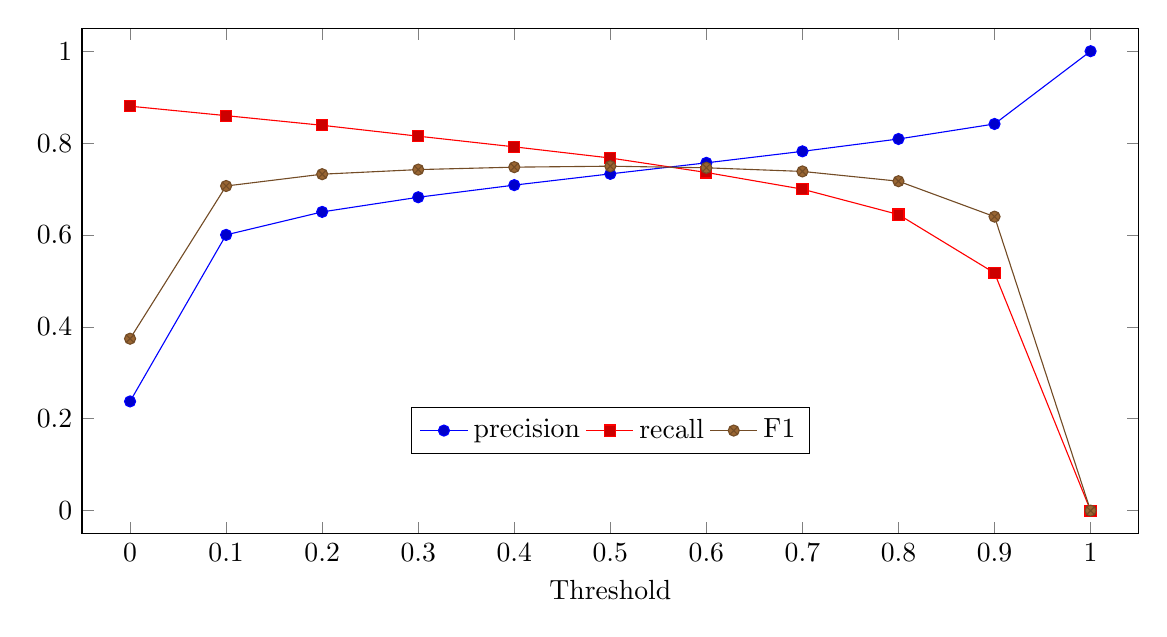
\begin{tikzpicture}
        \begin{axis}[
                height=8cm,
                width=15cm,
                xlabel=Threshold,
                legend style={at={(0.5,0.25)},
                anchor=north,legend columns=-1},
                enlarge x limits=0.05,
                enlarge y limits=0.05,
                xticklabel style={/pgf/number format/assume math mode},
                yticklabel style={/pgf/number format/assume math mode},
            ]
            \addplot+[sharp plot] coordinates
            {
                (0.0,0.2377)
                (0.1,0.6002)
                (0.2,0.6502) 
                (0.3,0.6821) 
                (0.4,0.7085) 
                (0.5,0.7330)
                (0.6,0.7570) 
                (0.7,0.7820) 
                (0.8,0.8089) 
                (0.9,0.8416) 
                (1.0,1.0000)};

            \addplot+[sharp plot] coordinates
            {
                (0.0,0.8803)
                (0.1,0.8597) 
                (0.2,0.8387) 
                (0.3,0.8150) 
                (0.4,0.7918) 
                (0.5,0.7675)
                (0.6,0.7360) 
                (0.7,0.6997) 
                (0.8,0.6445) 
                (0.9,0.5172) 
                (1.0,0.0000)};

            \addplot+[sharp plot] coordinates
            {
                (0.0,0.3742)
                (0.1,0.7066) 
                (0.2,0.7323) 
                (0.3,0.7423) 
                (0.4,0.7476) 
                (0.5,0.7497)
                (0.6,0.7462) 
                (0.7,0.7383) 
                (0.8,0.7170) 
                (0.9,0.6399) 
                (1.0,0.0000)};

            \legend{precision,recall,F1}
        \end{axis}
    \end{tikzpicture}
\caption{\label{i:classify-threshold} Performance for the pipeline system
with different thresholds. }
\end{figure}


Finally, we summarize our results for discourse disambiguation for
connective component instances in Table~\ref{t:recognition-methods}. We also
compare with various related work. The first two models are discourse disambiguation
on component level and on connective level without linking disambiguation. The following
models eliminate additional candidates by resolving linking ambiguity.
Some spurious candidates are removed in this process. However, it also removes some
correct components, so the resulting F1 score does not improve much.

%t:recognition-methods
\begin{table}[ht]
\centering
\begin{tabular}{|l|c|c|c|c|}
\hline

    Method                    &     Precision &     Recall &     F1-Score &     Accuracy \\ \hline
    @ w/o linking resolution  &     79.92     &     77.44  &     78.64    &     92.79    \\ \hline
    \# w/o linking resolution &     76.23     &     81.35  &     78.68    &     92.46    \\ \hline
    @len-score                & \bf 81.84     &     75.66  &     78.60    & \bf 92.96    \\ \hline
    \#len-score               &     77.27     &     80.45  &     78.81    &     92.61    \\

\hhline{|=|=|=|=|=|}

    Li et al. maximum entropy &     78.8      &     61.8   &     69.2     &     87.2     \\ \hline
    Li et al. decision tree   &     56.8      &     49.6   &     52.3     &     88.4     \\

\hhline{|=|=|=|=|=|}

    Zhou et al.               &               &            &     79.33    &     70.43    \\ \hline
    J. Jessy Li et al.        &     78.57     & \bf 81.48  & \bf 80.00    &     82.04    \\ \hline

\end{tabular}
\begin{flushleft}
\small
\textbf{@}: disambiguation on component level \\
\textbf{\#}: disambiguation on connective level \\
\end{flushleft}
\caption{\label{t:recognition-methods} Comparison for performance of discourse usage
disambiguation for connective component instances. }
\end{table}


Results from \cite{li2015automatic} are listed as they use the
same dataset as us. The best results for Maximum Entropy and Decision Tree classifiers with
automatic parsing tree features are selected. We use the 12,526 connective components candidates
extracted by string matching with connective lexicon as our basis to compute the accuracy in order
to compare with their work. Our models perform significantly better by a large margin.

We also list the results from \cite{zhou2012cross} and \cite{li2014cross} on different
datasets. Though it's not directly comparable with our work, the performance for F1 scores is similar,
and we have better accuracy.


\section{Discourse Relation Type Disambiguation}

\subsection{Relation Type Disambiguation for Known Connectives}

We will first evaluate our models using 10-fold cross-validation with the 1,813
explicit connectives. We divide them into 10 splits
while keeping the distribution for the relation types roughly equal for
each fold, and use Logistic Regression to classify the relation types.
Two sets of experiments for the four top-level
categories and the second-level categories are examined. The second-level categories
have 17 types, but there are three types (inference, background, and evaluation)
that have less than 10 instances. Therefore, we eliminate these instances and only evaluate
our models on the remaining 14 types. The resulting dataset contains 1,803 explicit
connectives. The macro-averaged
precision, recall, and F1 scores for different relation types and the accuracy for
all instances are computed. Finally, the averaged results over
the 10 folds are reported in Table~\ref{t:sense-features}.

We examined whether the same features
for connective candidates specified in Section~\ref{s:connective-features} are
also useful for relation type disambiguation. In addition, we use the string
of the connective itself as a feature. While the NUM features have some
discriminative power for discourse usage disambiguation on connective level,
it does not help for relation disambiguation. SKIPGRAM is still the most powerful
feature set.

%t:sense-features
\begin{table}[ht]
\centering
\begin{tabular}{|l|c|c|c|c|c|c|c|c|}
\hline
                  & \multicolumn{4}{c|}{4 Relation Types}      & \multicolumn{4}{c|}{17 Relation Types}                                    \\ \hline
\bf Features      & \bf P         & \bf R      & \bf F         & \bf A         & \bf P         & \bf R      & \bf F        & \bf A         \\ \hline
    P \& N        &     94.94     &     91.85  &     93.08     &     79.98     &     71.32     &     61.72  &     64.42    &     86.53     \\ \hline
    POS           &     85.66     &     70.47  &     75.10     &     82.79     &     34.51     &     31.12  &     31.76    &     68.58     \\ \hline
    NUM           &     13.42     &     24.97  &     17.46     &     53.67     &      8.24     &      7.27  &      4.99    &     41.27     \\ \hline
    SKIPGRAM      &     95.23     &     94.43  &     94.73     &     95.36     &     77.36     &     72.36  & \bf 73.40    &     89.02     \\ \hline
    CONNECITVE    &     94.94     &     91.85  &     93.08     &     94.16     &     71.32     &     61.72  &     64.42    &     86.53     \\ \hline
    All-P \& N    &     95.33     &     94.39  &     94.77     &     95.59     &     74.07     &     67.60  &     69.20    &     88.73     \\ \hline
    All-POS       &     95.51     &     94.12  &     94.70     &     95.36     &     71.04     &     66.31  &     67.42    &     88.13     \\ \hline
    All-NUM       & \bf 95.84     &     94.52  &     95.07     &     95.80     & \bf 75.69     & \bf 72.38  &     73.16    & \bf 89.23     \\ \hline
    All-SKIPGRAM  &     94.69     &     92.76  &     93.58     &     94.88     &     68.63     &     62.58  &     64.00    &     86.54     \\ \hline
    All-CONNECITVE&     95.44     &     94.47  &     94.86     &     95.64     &     71.77     &     66.15  &     67.50    &     88.30     \\ \hline
    All           &     95.77     & \bf 94.78  & \bf 95.18     & \bf 95.97     &     71.49     &     66.96  &     68.01    &     88.52     \\ \hline

\end{tabular}
\caption{\label{t:sense-features} Performance of relation type
disambiguation for connectives by different features. }
\end{table}



In Table~\ref{t:sense-types}, we show the performance for different relation types
using \textit{All-NUM} as features. For the second-level relation types, we only list
those types that have more than 10 instances. We could notice that the
number of instances affects the performance of the learning model. The
lesser the instances, the worse the performance.

%t:sense-types
\begin{table}[ht]
\centering
\begin{tabular}{|l|c|c|c|c|}
\hline

\multicolumn{5}{|c|}{4 Relation Types}                                              \\ \hline
    Features            &     Precision &     Recall &     F1-Score &     Instances \\ \hline
    causality           &     96.34     &     95.04  &     95.61    &     465       \\ \hline
    coordination        &     95.75     &     97.23  &     96.45    &     974       \\ \hline
    transition          &     93.72     &     91.31  &     92.34    &     173       \\ \hline
    explanation         &     97.54     &     94.50  &     95.88    &     201       \\ \hline
    macro-AVG           &     95.84     &     94.52  &     95.07    &     1813      \\ \hline

\multicolumn{5}{|c|}{14 Relation Types}                                             \\ \hline
    Features            &     Precision &     Recall &     F1-Score &     Instances \\ \hline
    cause-result        &     89.71     &     94.57  &     91.98    &     203       \\ \hline
    hypothetical        &     92.17     &     86.00  &     88.65    &     55        \\ \hline
    purpose             &     94.18     &     88.27  &     90.91    &     163       \\ \hline
    condition           &     75.50     &     66.67  &     68.60    &     37        \\ \hline
    coordination        &     88.10     &     96.22  &     91.95    &     741       \\ \hline
    continue            &     84.22     &     74.18  &     78.35    &     133       \\ \hline
    progressive         &     84.50     &     55.67  &     65.25    &     52        \\ \hline
    selectional         &     50.00     &     50.00  &     50.00    &     10        \\ \hline
    inverse             &     76.67     &     28.33  &     39.71    &     38        \\ \hline
    transition          &     92.00     &     91.17  &     91.46    &     157       \\ \hline
    concessive          &     80.00     &     75.00  &     76.67    &     16        \\ \hline
    explanation         &     55.00     &     60.00  &     56.67    &     11        \\ \hline
    summary-elaboration &     99.38     &     98.12  &     98.73    &     158       \\ \hline
    example             &     87.50     &     90.00  &     87.90    &     29        \\ \hline
    macro-AVG           &     82.07     &     75.30  &     76.92    &     1803      \\ \hline

\end{tabular}
\caption{\label{t:sense-types} Performance of relation type
disambiguation. }
\end{table}


We also evaluate on component instances to compare with \cite{li2015automatic}.
We are able to achieve higher performance on relation type classification.

%t:sense-word-types
\begin{table}[!htbp]
\centering
\begin{tabular}{|l|c|c|c|c|c|c|}
\hline

                        & \multicolumn{3}{c|}{our model}            & \multicolumn{3}{c|}{Li et al.}            \\ \hline
    Type                &     Precision &     Recall &     F1-Score &     Precision &     Recall &     F1-Score \\ \hline
    causality           &     95.84     &     94.20  &     94.90    &     83.8      &     68.4   &     75.1     \\ \hline
    coordination        &     95.66     &     97.34  &     96.45    &     82.5      &     93.6   &     87.7     \\ \hline
    transition          &     95.04     &     91.78  &     93.18    &     78.5      &     59.6   &     67.0     \\ \hline
    explanation         &     97.54     &     94.07  &     95.63    &     89.7      &     82.8   &     85.9     \\ \hline

\end{tabular}
\caption{\label{t:sense-word-types} Performance of relation type
disambiguation for component instances. }
\end{table}


\subsection{Relation Type Disambiguation within the Pipeline System}

We also evaluate discourse relation disambiguation within the pipeline system
using the \textit{\#+len+score} model.
For each connective candidate extracted, we predict its relation type using
Logistic Regression with \textit{All-NUM} as features.
The same 10-fold for paragraphs is used, and the precision, recall, and F1 scores
for positive instances are computed. The results are listed in
Table~\ref{t:sense-types-pipeline}. The micro-averaged F1 72.64\% can be seen
as the ability for our model to propose connective candidates along with the correct
relation type. Compared with the original F1 score 74.97\% disregarding relation types,
the performance only decreases a little, showing the effectiveness of our
model for relation type disambiguation.

%t:sense-types-pipeline
\begin{table}[ht]
\centering
\begin{tabular}{|l|c|c|c|c|}
\hline

\multicolumn{5}{|c|}{4 Relation Types}                                              \\ \hline
\bf Features            & \bf Precision & \bf Recall & \bf F1-Score & \bf Instances \\ \hline
    causality           &     69.98     &     75.37  &     72.24    &     465       \\ \hline
    coordination        &     67.70     &     70.63  &     69.09    &     974       \\ \hline
    transition          &     80.75     &     76.31  &     78.25    &     173       \\ \hline
    explanation         &     80.84     &     89.27  &     84.49    &     201       \\ \hline
    macro-AVG           &     74.82     &     77.90  &     76.02    &     1813      \\ \hline
    micro-AVG           &     71.13     &     74.48  &     72.75    &     1813      \\ \hline

\end{tabular}
\caption{\label{t:sense-types-pipeline} Performance of relation type
disambiguation within the pipeline system. }
\end{table}


\section{Connective Argument Extraction}

\subsection{Connective Argument Extraction for Known Connectives}

In this section, we discuss our evaluation on argument extraction when the
positions of connectives are already known.

We will use the same 10-fold for paragraphs for evaluation.
The precision, recall, and F1 scores for the argument boundaries are
computed for each fold. Additionally, we also compute the accuracy among the 
connectives. Each connective is treated as an instance, and we only count it
as correct if all argument boundaries for the given connective are correctly identified.
The averaged results over all folds are reported. Table~\ref{t:argument-features} shows
the performance using different feature sets.

While the best F1 score for connective boundaries is 78.48\%, the accuracy for
the connectives is only 40.74\%, showing a lot of spaces for
improvement. It means that for each connective, we are able to recover most of its
argument boundaries, but it's difficult to recover all of them correctly.

%t:argument-features
\begin{table}[ht]
\centering
\begin{tabular}{|l|c|c|c|c|}
\hline

    Features        &     Precision &     Recall &     F1-Score                 &     Connective Accuracy \\ \hline
    CONTEXT         &     52.25     &     30.30  &     38.35\textsuperscript{*} &      1.89               \\ \hline
    PATH            &     76.60     &     56.45  &     64.97\textsuperscript{*} &     14.71               \\ \hline
    POS             &     55.76     &     38.56  &     45.56\textsuperscript{*} &      7.34               \\ \hline
    SUBJ            & \bf 88.00     &      7.88  &     14.40\textsuperscript{*} &      0.00               \\ \hline
    ENDCHAR         &     46.06     &     29.74  &     36.14\textsuperscript{*} &      0.00               \\ \hline
    LINK            &     76.90     &     40.01  &     52.61\textsuperscript{*} &      1.83               \\ \hline
    CONNECTIVE      &     46.95     &     30.46  &     36.95\textsuperscript{*} &      0.49               \\ \hline
    COMPONENT       &     68.84     &     66.98  &     67.89\textsuperscript{*} &     21.90               \\ \hline
    All-CONTEXT     &     79.15     &     75.75  &     77.41\textsuperscript{*} &     38.38               \\ \hline
    All-PATH        &     78.41     &     74.47  &     76.38\textsuperscript{*} &     35.69               \\ \hline
    All-POS         &     76.79     &     74.40  &     75.57\textsuperscript{*} &     35.60               \\ \hline
    All-SUBJ        &     80.14     &     76.62  &     78.34\textsuperscript{ } &     39.97               \\ \hline
    All-ENDCHAR     &     80.14     &     76.58  &     78.32\textsuperscript{*} &     40.41               \\ \hline
    All-LINK        &     80.03     &     76.71  &     78.33\textsuperscript{*} &     40.25               \\ \hline
    All-CONNECTIVE  &     79.62     &     75.82  &     77.67\textsuperscript{*} &     37.94               \\ \hline
    All-COMPONENT   &     74.98     &     60.80  &     67.13\textsuperscript{*} &     21.68               \\ \hline
    All             &     80.24     & \bf 76.80  & \bf 78.48\textsuperscript{!} & \bf 40.74               \\ \hline

\end{tabular}
\caption{\label{t:argument-features} Performance of argument boundary detection
using different features. }
\end{table}


We compare our model with a simple baseline model. The model places an argument
boundary at the beginning of each segment that contains a connective component for
the current connective. In addition, it places an argument boundary at the
end of the segment that contains the last connective component. If the connective
has only one component, only two boundaries are placed, so we place an additional
boundary after the last boundary or before the first boundary if
the last boundary is already the end of the paragraph. The results are shown
in Table~\ref{t:argument-baseline}. Our model outperforms the baseline model
significantly.

%t:argument-baseline
\begin{table}[!htbp]
\centering
\begin{tabular}{|l|c|c|c|c|}
\hline

    Method          &     Precision &     Recall &     F1-Score &     Connective Accuracy \\ \hline
    our model       & \bf 80.24     & \bf 76.80  & \bf 78.48    & \bf 40.74               \\ \hline
    baseline        &     23.83     &     28.90  &     26.12    &      3.04               \\ \hline

\end{tabular}
\caption{\label{t:argument-baseline} Comparison for performance of argument boundary detection. }
\end{table}


\subsection{Error Analysis}

We continue to analyze the errors produced by our model.
Figure~\ref{i:argument-error-len} shows the distribution of the number
of arguments and the number of connective components for each explicit discourse
relation and the respective error rates measured by connective accuracy.
Our model can mostly only handle the relations
that only have two arguments. For more arguments, the error rates are almost
close to 1. We also examine whether it's important for
the number of arguments and the number of component to match as shown in
Figure~\ref{i:argument-error-len-c}, but no significant difference is observed.

%i:argument-error-len
\begin{figure}[ht]
\begin{subfigure}{.4\textwidth}
    \centering
    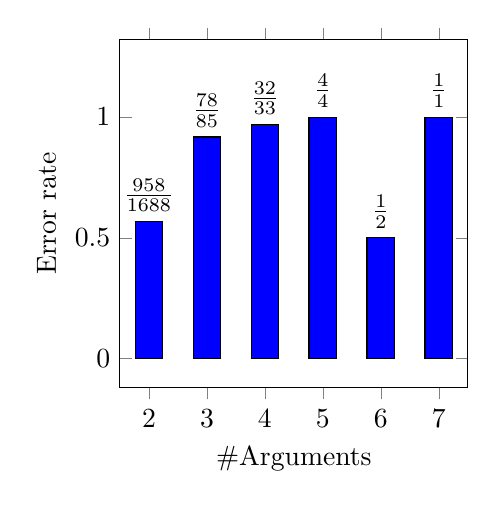
\begin{tikzpicture}
        \begin{axis}[
            enlarge y limits=0.1,
            enlarge x limits=0.1,
            width=6cm,
            height=6cm,
            xtick={2,...,7},
            ymin=0,
            ymax=1.2,
            ybar,
            ylabel=Error rate,
            xlabel=\#Arguments,
            nodes near coords,
            xtick=data
          ]
            \addplot[ybar,fill=blue,point meta=explicit symbolic] coordinates {
            (2,958/1688) [$\frac{958}{1688}$]
            (3,78/85) [$\frac{78}{85}$]
            (4,32/33) [$\frac{32}{33}$]
            (5,4/4)   [$\frac{4}{4}$]
            (6,1/2)   [$\frac{1}{2}$]
            (7,1/1)   [$\frac{1}{1}$]
            };
        \end{axis}
    \end{tikzpicture}
    \caption{Error rates by the number of arguments each connective has.}
    \label{i:argument-error-len-a}
\end{subfigure}
\begin{subfigure}{.4\textwidth}
    \centering
    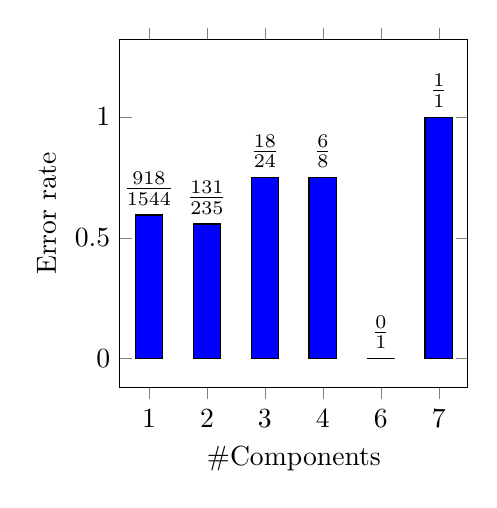
\begin{tikzpicture}
        \begin{axis}[
            enlarge x limits=0.1,
            enlarge y limits=0.1,
            width=6cm,
            height=6cm,
            xticklabels={1,2,3,4,6,7},
            xtick={1,2,...,6},
            ymin=0,
            ymax=1.2,
            ybar,
            ylabel=Error rate,
            xlabel=\#Components,
            nodes near coords,
            xtick=data
          ]
            \addplot[ybar,fill=blue,point meta=explicit symbolic] coordinates {
            (1,918/1544) [$\frac{918}{1544}$]
            (2,131/235) [$\frac{131}{235}$]
            (3,18/24) [$\frac{18}{24}$]
            (4,6/8)   [$\frac{6}{8}$]
            (5,0/1)   [$\frac{0}{1}$] %6
            (6,1/1)   [$\frac{1}{1}$] %7
            };
        \end{axis}
    \end{tikzpicture}
    \caption{Error rates by the number of components each connective has.}
    \label{i:argument-error-len-b}
\end{subfigure}
\begin{subfigure}{1\textwidth}
    \centering
    \vspace{2em}
    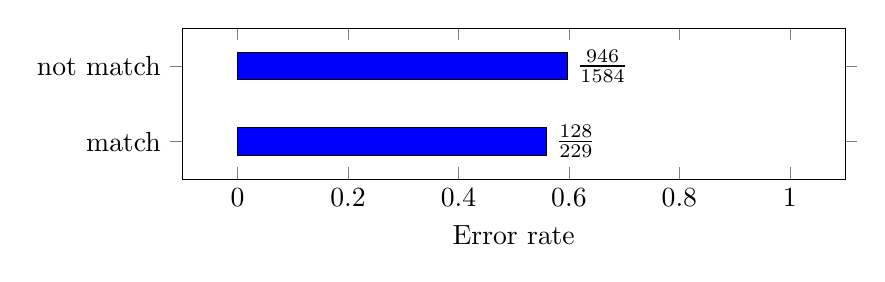
\begin{tikzpicture}
        \begin{axis}[
            enlarge y limits=0.5,
            enlarge x limits=0.1,
            height=3.5cm,
            width=10cm,
            yticklabels={match, not match},
            ytick={1,2},
            xmin=0,
            xmax=1,
            xbar=1pt,
            xlabel=Error rate,
            nodes near coords,
            nodes near coords align={horizontal},
            every node near coord/.append style={
                anchor=west}
            ,
            ytick=data
          ]
            \addplot[xbar,fill=blue,point meta=explicit symbolic] coordinates {
            (128/229,1) [$\frac{128}{229}$]
            (946/1584,2) [$\frac{946}{1584}$]
            };
        \end{axis}
    \end{tikzpicture}
    \caption{Error rates by whether \#Arguments is the same as \#Components
        in each relation.}
    \label{i:argument-error-len-c}
\end{subfigure}
    \vspace{1em}
    \caption{\label{i:argument-error-len} Error rates for argument extraction
        grouped by different criteria. }
\end{figure}


The arguments for an explicit discourse relation span over a continuous argument interval
that starts from the first argument boundary and ends at the last argument boundary.
There exist four types of relationships between the real interval and the predicted
interval as shown in Figure~\ref{i:args-relationship}.

%i:args-relationship
\begin{figure}[!htbp]
\centering

superset
\vspace{0.2em}
{\large
\[
\begin{array}{*8{c}}
(a)&(b)&\underscope{predicted}{(c)&\overscope{real}{(d)&(e)&(f)&(g)&(h)}}
\end{array}
\]
}
\vspace{0.5em}

subset
\vspace{0.2em}
{\large
\[
\begin{array}{*8{c}}
(a)&(b)&(c)&\overscope{real}{(d)\underscope{predicted}{&(e)&(f)&(g)&(h)}}
\end{array}
\]
}
\vspace{0.5em}

intersect
\vspace{0.2em}
{\large
\[\def\arraystretch{0.0}
\begin{array}{*8{c}}
(a)&(b)&(c)&\overscope{real}{(d)&(e)&(f)&(g)&(h)}\\[-1em]
\hphantom{(a)}&\hphantom{(b)}&\underscope{predicted}
{\hphantom{(c)}&\hphantom{(d)}&\hphantom{(e})&\hphantom{(f})&
\hphantom{(g)}}&\hphantom{(h)}
\end{array}
\]
}
\vspace{0.5em}

exact
\vspace{0.2em}
{\large
\[
\begin{array}{*8{c}}
(a)&(b)&(c)&\underscope{predicted}{\overscope{real}{(d)&(e)&(f)&(g)&(h)}}
\end{array}
\]
}
\vspace{0.5em}

\caption{\label{i:args-relationship} Relationships between real argument intervals
and predicted intervals. }

\end{figure}


We examine the distribution of the errors for these types of relationships and the
results are shown in Figure~\ref{i:argument-error-type}. We found in most cases,
the interval predicted is either too wide or too narrow.
Only 139 error cases are caused entirely by the argument boundaries within the
interval. The difficulty to determine the argument interval originates from
the large variety for the ranges of explicit relations. For the relations that
are represented by higher nodes in the discourse tree,
the range is so wide that it could contain almost the entire paragraph.
On the other hand, some relations only span over one part of a sentence.

%i:argument-error-type
\begin{figure}[ht]
    \centering
    \vspace{2em}
    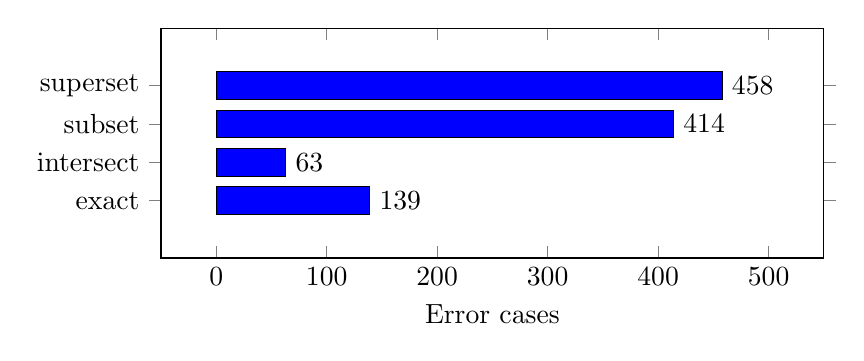
\begin{tikzpicture}
        \begin{axis}[
            enlarge y limits=0.5,
            enlarge x limits=0.1,
            height=4.5cm,
            width=10cm,
            symbolic y coords={
            exact,intersect,subset,superset
            },
            xmin=0,
            xmax=500,
            xbar=1pt,
            xlabel=Error cases,
            nodes near coords={\pgfmathprintnumber[/pgf/number format/assume math mode]{\pgfplotspointmeta}},
            nodes near coords align={horizontal},
            every node near coord/.append style={
                anchor=west}
            ,
            xticklabel style={/pgf/number format/assume math mode},
            yticklabel style={/pgf/number format/assume math mode},
            ytick=data
          ]
            \addplot[xbar,fill=blue] coordinates {
            (458,superset)
            (414,subset)
            (63,intersect)
            (139,exact)
            };
        \end{axis}
    \end{tikzpicture}
    \caption{\label{i:argument-error-type} Error cases for argument extraction
        by the relationship with the real interval. }
\end{figure}


Intriguingly, there are only 63 \textit{intersect} cases. Further investigation
reveals that in most cases, at least one side of the interval is correctly
identified. This is shown in Figure~\ref{i:argument-error-position}. Out of
the 1074 error cases, there are only 164 cases that the both sides of the
interval are incorrect. The reason behind this is probably due to the fact that
the existence of a connective often gives strong hint on at least one side of
the interval. On the contrary, there is often no explicit indication on the boundary
of the other side of the interval.

%i:argument-error-position
\begin{figure}[ht]
    \centering
    \vspace{2em}
    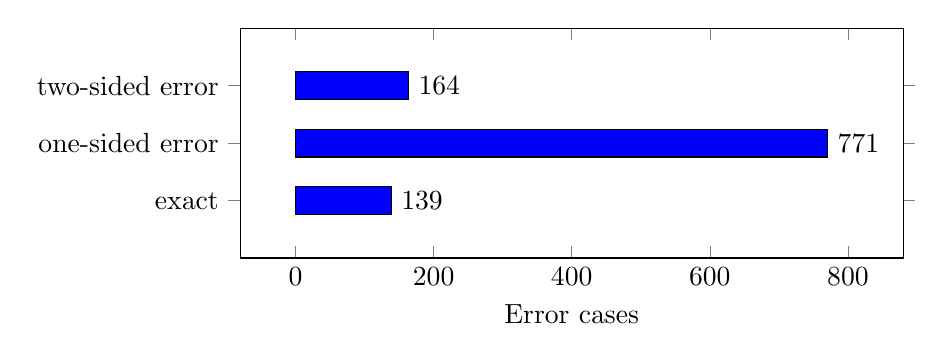
\begin{tikzpicture}
        \begin{axis}[
            enlarge y limits=0.5,
            enlarge x limits=0.1,
            height=4.5cm,
            width=10cm,
            symbolic y coords={
            exact,one-sided error,two-sided error
            },
            xmin=0,
            xmax=800,
            xbar=1pt,
            xlabel=Error cases,
            nodes near coords,
            nodes near coords align={horizontal},
            every node near coord/.append style={
                anchor=west}
            ,
            ytick=data
          ]
            \addplot[xbar,fill=blue] coordinates {
            (139,exact)
            (771,one-sided error)
            (164,two-sided error)
            };
        \end{axis}
    \end{tikzpicture}
    \caption{\label{i:argument-error-position} Error cases for argument extraction
        by the first and last boundaries. }
\end{figure}


\subsection{Connective Argument Extraction within the Pipeline System}

Once argument extraction is integrated into the pipeline system, our end-to-end
pipeline would be able to extract explicit relations for raw text. In particular,
it proposes a set of explicit relation candidates, where each relation contains
three items: (1) the positions of the connective, (2) the relation type, and
(3) the arguments. \textit{\#+len+score} is used for connective extraction, and
\textit{All-NUM} is used to disambiguate 4 top-level relation types.
We use the same 10-fold for paragraphs to evaluate our model using each relation
as an instance. The precision, recall, and F1 scores are computed for each fold,
and the averaged results are reported. Each explicit relation candidate is
counted as true positive only when the three items are all correctly
identified; otherwise, it is counted as false positive. We list the results
in Table~\ref{t:final-results}. We could see that due to the difficulty
of argument extraction, the performance has decreased significantly compared
to the previous stage. We additionally list the performance of end-to-end
parsers reported by \cite{lin2014pdtb} and \cite{kong2014a}. Their results
were also evaluated on the F1 for the relations extracted.
However, their works include the identification of implicit relations while
our system focuses only on explicit relations.
Also, as they used PDTB2, the language and annotation standard are different from
ours, so it's not actually directly comparable.

%t:final-results
\begin{table}[ht]
\centering
\begin{tabular}{|c|c|c|c|}
\hline

Method      &    Precision &     Recall &     F1-Score \\ \hline
our model   &    30.59     &     32.07  &     31.31    \\ \hline
Lin et al.  &              &            &     20.64    \\ \hline
Kong et al. &              &            &     27.39    \\ \hline


\end{tabular}
\caption{\label{t:final-results} Final performance of our pipeline system. }
\end{table}

